\section*{asnwers}
1. The neutron decay width predominantly depends on quantities such as: $\Delta$, $G_\beta$
\begin{equation}
\begin{split}
&\Gamma = \frac{1}{60\pi^3}G_\beta^2 \Delta ^5
\end{split}
\end{equation}
$\Delta$ is maximal energy of produced electron: 
\begin{equation}
\begin{split}
&\Delta =\frac{m_n^2-(m_p+m_\nu)^2+m_e^2}{2m_n}\approx m_n-m_p=1.29 MeV\\
&G_\beta = 1.136*10^{-5}GeV^{-2}\\
\end{split}
\end{equation}
Also, parameter $f=1.27$ which accounts for non-elementary structure of neutron.
\begin{equation}
\begin{split}
&\mathcal{L}_{int}^\beta=-\frac{G_\beta}{\sqrt{2}}[\Bar{\psi}_p\gamma^\mu (1-f\gamma_5)\psi_n][\Bar{\psi}_e\gamma_\mu (1-\gamma_5)\psi_{\nu_e}]
\end{split}
\end{equation}
2. The neutron decay width predominantly depends on quantities such as: $\Delta\approx m_\mu$, $G_\mu$
$\Delta$, $G_\beta$
\begin{equation}
\begin{split}
&\Gamma = \frac{1}{192\pi^3}G_\mu^2 m_\mu ^5\\
&m_\mu = 105 MeV\\
&G_F=G_\mu=1.16638*10^{-5} GeV^{-2}
\end{split}
\end{equation}
\begin{equation}
\begin{split}
&\mathcal{L}_{int}^\mu=-\frac{G_\mu}{\sqrt{2}}[\Bar{\psi}_{\nu_\mu}\gamma^\mu (1-\gamma_5)\psi_\mu][\Bar{\psi}_e\gamma_\mu (1-\gamma_5)\psi_{\nu_e}]
\end{split}
\end{equation}
$G_F>G_\beta$.

3. The reason behind the substantial difference between the lifetimes of the muon ($10^{-6}\ s$) and the neutron ($880 \ s$) is big difference in maximal energies of produced electron. 

4. Approximately, the maximum energy of the electron in the neutron beta decay is $\Delta =\frac{m_n^2-(m_p+m_\nu)^2+m_e^2}{2m_n}\approx m_n-m_p=1.29 MeV$. If neutron is static and proton is quasi-static. Mass of electron is $0.51 \ MeV$. So, $\gamma$ is: $E = m \cdot \gamma$: $\gamma=2.58$ and $\beta$ is : $\beta=0.921829$ - so, quite relativistic. No, maximal energy of proton would be: $E_p=\frac{m_n^2+m_p^2-(m_e+m_\nu)^2}{2m_n}=m_n$, so $\gamma=1$ and $\betas=0$.

5. The dimension of Fermi constant is $GeV^{-2}$: from the dimension calculation of Lagrangian of beta decay. $G_F=G_\mu=1.16638*10^{-5} GeV^{-2}$.

6. From PDG we see: $BR(\pi^- \rightarrow \mu^- + \Bar{\nu}_\mu )\approx 99.9877\%$ and $BR(\pi^- \rightarrow e^- + \Bar{\nu}_e )\approx 1.23*10^{-4}\%$
\begin{equation}
\begin{split}
&\mathcal{L}_{int}^{eff}=F \partial_\mu \phi^- [\psi_l \gamma^\mu (1-\gamma_5)\psi_{\nu_l}]\\
&\frac{\Gamma(\pi^- \rightarrow e^- + \Bar{\nu}_e )}{\Gamma(\pi^- \rightarrow \mu^- + \Bar{\nu}_\mu )}=\frac{m_e^2(m_\pi^2-m_e^2)^2}{m_\mu^2(m_\pi^2-m_\mu^2)^2}=1.3*10^{-4}\\
\end{split}
\end{equation}
Electron mode is suppressed. 

7.The label V-A in the theory of Weak interactions: that from vector current of fermions we subtract the axial vector fermion current. We use such combination due to parity violation, which was discovered by Lee and Yang in 1957.

8. $CP$ and $CPT$ are exact, $P$ and $C$ are violated.

9. $G_F=G_\mu>G_\beta$.

10. $G_F=G_\mu>G_\beta>G_\Sigma$. There exact relations: $G_\Sigma = G_F \sin \theta_C$ and $G_\beta = G_F \cos \theta_C$ for $\theta_C=13'$. When strangeness is changed, we use sin otherwise: cos.
11. The energy dependence of the cross-section for neutrino-electron scattering in the HEL within Fermi-type theory:
\begin{equation}
\begin{split}
&\sigma^{(\nu e)}=\frac{G_F^2}{\pi}s
\end{split}
\end{equation}
12. The HEL asymptotics of $\nu-e$ scattering cross-section evaluated within IVB and Fermi-type model differ in such way:
\begin{equation}
\begin{split}
&\sigma^{\nu e}_{IVB}=\frac{G_F^2}{\pi}m_W^2\\
&\sigma^{(\nu e)}_{Fermi}=\frac{G_F^2}{\pi}s\\
\end{split}
\end{equation}

13. The relation between parameters of Fermi model and IVB one:
\begin{equation}
\begin{split}
&\frac{G_F}{\sqrt{2}}=\frac{g^2}{8m_W^2}
\end{split}
\end{equation}

14. The process of electron-positron annihilation into production of a $WW$ pair in the IVB model has 2 possible diagrams in tree level: where electron emits $W^-$ and turns into neutrino propagator and emits $W^+$ and becomes positron. And second one is when electron and positron annihilate into photon which decays to $W^+W^-$ pair. Matrix elemts are as follows for limit of longitudinal:
\begin{equation}
\begin{split}
&M^\nu_{e^-e^+} = \frac{-g^2}{4m_W^2}\Bar{v}(l)\slashed{p}(1-\gamma_5)u(k)+O(\frac{m_e}{m_W^2}E)+O(1)\\
&M^\gamma_{e^-e^+} = \frac{e^2}{m_W^2}\Bar{v}(l)\slashed{p}u(k)+O(1)\\
\end{split}
\end{equation}
These two matrix elements cannot be cancelled only working in IVB theory b.c of presence of $\gamma_5$. If final states are not longitudinal or are averaged, then $M\approx O(1)$. In case of non-Abelian fields (when there is a neutral boson particles $Z$-bosons, which interact with $W$-bosons) the sum of these diagrams acts as O(E), and after introducing Higgs boson, this process is of order O(1).

15. The high-energy behaviour of the longitudinal polarization of a massive vector boson is: 
\begin{equation}
\begin{split}
&\varepsilon_\mu(p_0,\Vec{p}) = (\frac{|\Vec{p}|}{m},\frac{p_0}{m}\frac{\Vec{p}}{|\Vec{p}|}) |_{HEL} \approx \frac{p_\mu}{m}+O(\frac{m}{p_0})\\
\end{split}
\end{equation}

16. The main difference between the Lagrangian's of the Yang-Mills field and the case of the Maxwell electromagnetic fields is that free part of Lagrangian for gauge field has self-interactions of type: $AAA$ and $AAAA$:
\begin{equation}
\begin{split}
&\mathcal{L}_{YM} = -\frac{1}{4}G^a_{\mu\nu}G^{a\mu\nu}\\
&G^a_{\mu\nu} =\partial_\mu A_\nu^a - \partial_\nu A_\mu^a +g\varepsilon^{abc}A^b_{\mu}A^c_{\nu}\\
&\mathcal{L}_{em} = -\frac{1}{4}F_{\mu\nu}F^{\mu\nu}\\
&F^a_{\mu\nu} =\partial_\mu B_\nu^a - \partial_\nu B_\mu^a \\
\end{split}
\end{equation}

17. The gauge group of the Standard Model of electroweak interactions is $SU(2)\times U(1)$.

18. Covariant derivative is such that under transformation of group, transforms as: $D_\mu\rightarrow D_\mu^{'} = S D_\mu S^{-1}$, where $\psi\rightarrow \psi^{'}=S\psi$
\begin{equation}
\begin{split}
&S=e^{i w^a T^a}\\
&[T^a,T^b]=if^{abc}T^c\\
&D_\mu = \partial_\mu - i g A_\mu\\
&A_\mu'= SA_\mu S^{-1}+\frac{i}{g} S\partial _\mu S^{-1}\\
\end{split}
\end{equation}
Where fields $A_\mu^a$ were introduced in order to cancel out phases $w^a$.

19. $F_{\mu\nu}$ has a connection to a covariant derivative such as:

\begin{equation}
\begin{split}
&-igF_{\mu\nu}=[D_\mu,D_\nu]\\
\end{split}
\end{equation}

20. The physical vector fields in SM related to the original gauge fields with following relationships:
\begin{equation}
\begin{split}
&W^+_\mu=A^-_\mu = \frac{1}{\sqrt{2}}(A_\mu^1 - i A_\mu^2) \\
&W^-_\mu=A^+_\mu = \frac{1}{\sqrt{2}}(A_\mu^1 + i A_\mu^2) \\
&A^3_\mu = \cos \theta _W Z_\mu +\sin \theta_W A_\mu\\
&B_\mu = -\sin \theta _W Z_\mu +\cos \theta_W A_\mu\\
\end{split}
\end{equation}

21. Neutral current is a more general form of $V-A$. Such that, $V$ and $A$ have their own respective coefficients. 
\begin{equation}
\begin{split}
&J_{NC}^\mu = \frac{g}{2\cos\theta_W}(\Bar{f} \gamma^\mu (v_f-a_f\gamma_5)f)\\
&v_f= \varepsilon_L^f + \varepsilon_R^f\\
&a_f= \varepsilon_L^f - \varepsilon_R^f\\
&\varepsilon_{L/R}^f=T_{3,L/R}^f -Q^f \sin^2 \theta_W\\
\end{split}
\end{equation}
Where f is a fermion particle, with specific third component isospin and charge. For neutrino $a=v=\frac{1}{2}$. For electron, muon, tau: $a=-\frac{1}{2}$ and $v=-\frac{1}{2}+2\sin^2 \theta_W$. Reminder: $\mathbb{L}=(\nu_L,e_L)$.

22. An example of neutral current is neutrino-electron scattering. Neutrino must be of other type, or there could be other processes, not necessarily the neutral current interaction. Also, such cross-sections are very small. Considering the total cross-section as a function of $\sin^2 \theta_W$, we can build plot of factor R:
\begin{equation}
\begin{split}
&R(\sin^2 \theta_W)=\frac{\sigma( \nu_\mu +e\rightarrow \nu_\mu +e )  }{\sigma( \Bar{\nu}_\mu +e\rightarrow \Bar{\nu}_\mu +e )}
\end{split}
\end{equation}
From experiment it was measured: $R\approx 1.2$ and $\sin^2 \theta_W=0.232$. From this we get: $\theta_W=28.8'$

23. The unification condition in SM is $e=g\sin \theta_W$. Knowing $\frac{G_F}{\sqrt{2}}=\frac{g^2}{8 m_W^2}$ using unif cond: $m_W^2=\frac{e^2}{4\sqrt{2} G_F\sin^2\theta_W}$ and $\alpha = \frac{e^2}{4\pi}=\frac{1}{137}$: $m_W = \sqrt{\frac{\pi\alpha}{\sqrt{2}G_F\sin^2\theta_W}}$, we get: $m_W\approx 77\ GeV$, which is close to measured at ATLAS $80.37\ GeV$. Using the fact, that maximum value of $\sin \theta $ is $1$, we can have a lower bound on mass of $W$-boson: $m_W > 37 \ GeV$.

24. There will be 3  diagrams. Exchange of neutrino, $Z$-boson and $\gamma$ exchange. The technical role of $Z$ is to cancel out $O(E^2)$ dependence of diagrams. 
\begin{figure}[H]
\centering
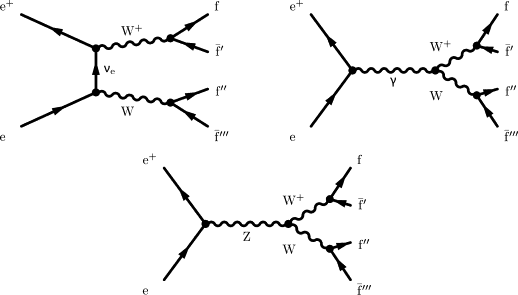
\includegraphics[width=\textwidth]{Images/ElectronPositronAnnihilationToWBosons}
\caption{Diagrams of electron positron annihilation to $W$-boson pair}
\end{figure}

25. The HEL behaviour of $W$-boson pair scattering is proportional to $O(E^2)$.
\begin{figure}[H]
\centering
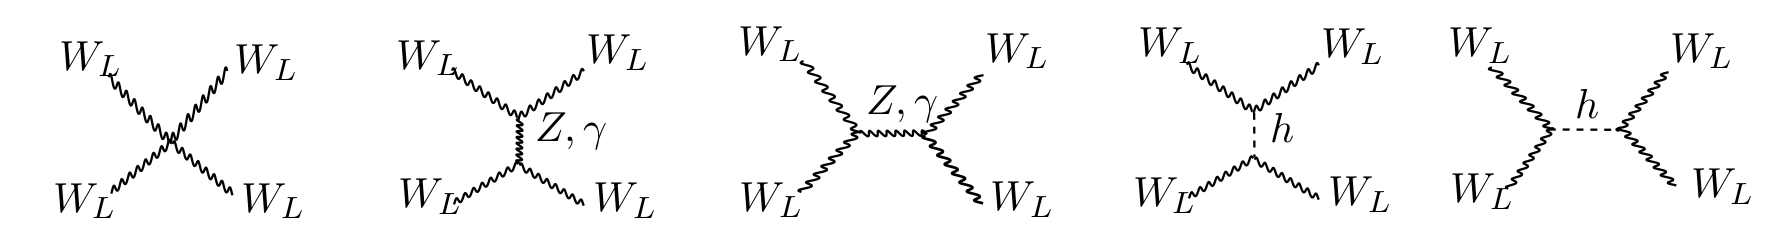
\includegraphics[width=\textwidth]{Images/WLWL.png}
\caption{Diagrams of $W$-boson pair scattering. Currently, we have not introduced Higgs particle. For $Z$ and $\gamma$ exchange, we have two diagrams: $u$ and $t$ modes}
\end{figure}

26. Possible interactions of vector bosons within SM are:
\begin{equation}
\begin{split}
&\mathcal{L}_{WW\gamma}\\
&\mathcal{L}_{WWZ}\\
&\mathcal{L}_{WW\gamma\gamma}\\
&\mathcal{L}_{WWWW}\\
&\mathcal{L}_{WWZZ}\\
&\mathcal{L}_{WWZ\gamma}\\
\end{split}
\end{equation}\

27. We start with four massless gauge fields and we want to end up with $3$ fields with masses and $1$ massless. It meands we want to break $3$ symmetry generators and 1 to be preserved. Combination of $SU(2)$ gives us desired number of broken and unbroken generators. Also, we want this scalar field to be non-trivially coupled to gauge $SU(2)$ fields. 

28. The $U$-gauge is a specific choice of phase-calibration to completely eliminate the angular field (or just a field). So, it is a certain gauge transformation out of infinity of such. 

29. The relation between masses of $Z$-boson and $W$-boson is as follow: $m_W = \cos \theta _W m_Z$ $m_W^2=\frac{1}{4}v^2 g^2$  $m_Z^2=\frac{1}{4}(g^2+g'^2)v^2$.

30. Using two relations:

\begin{equation}
\begin{split}
&m_W = \sqrt{\frac{\pi\alpha}{\sqrt{2}G_F\sin^2\theta_W}}\\
&m_W = \cos\theta_W m_Z\\
\end{split}
\end{equation}
We get:
\begin{equation}
\begin{split}
&m_Z  =\sqrt{\frac{\pi\alpha}{\sqrt{2}G_F}}\frac{1}{\sin\theta_W \cos\theta_W}=2\sqrt{\frac{\pi\alpha}{\sqrt{2}G_F}}\frac{1}{\sin2\theta_W } \\
\end{split}
\end{equation}
We get lower bound on mass of $Z$-boson: $37\cdot 2\ GeV\approx 74 \ GeV$.

31. The vacuum value $v$ of the Higgs field can be expressed as such: $v=(\sqrt{2}G_F)^{-\frac{1}{2}}\approx 246\ GeV$. 

32. Possible types of interactions of Higgs boson with vector bosons are: $WWH$, $ZZH$, $WWHH$ and $WWHH$. Explicit form of intereaction for $WWH$ is:
\begin{equation}
\begin{split}
&\mathcal{L}_{WWH}=g m_W W^-_\mu W^{+\mu}H
\end{split}
\end{equation}

33. There are 2 ways Higgs can self-interact:
\begin{equation}
\begin{split}
&\mathcal{L}_{HHH} = -\lambda v H^3\\
&\mathcal{L}_{HHHH} = -\frac{\lambda}{4}  H^4 \\
\end{split}
\end{equation}

34. Theoretical role of Higgs boson exchange in $WW$ scattering is to cancel out next leading order of divergences of $O(E^2)$. So, that matrix element behave as $O(1)$.

35. Lepton masses are generated through Yukawa coupling of fermion fields and Higgs field. With simple interaction Lagrangian of form: 
\begin{equation}
\begin{split}
&\mathcal{L}_{Yukawa} = - h_e \mathbb{L} \Phi e_R +h.c.
\end{split}
\end{equation}
After fixing $U$-gauge and contraction, we get: $m_e = \frac{v h_e}{\sqrt{2}}$. And we can generalize for all leptons in SM. 

36. 
\begin{equation}
\begin{split}
&
\end{split}
\end{equation}


